\documentclass{beamer}

\usepackage{txfonts}
\usepackage{hyperref}
\usepackage{fancybox}
\usepackage{xfrac}
\usepackage{cancel}


\newcommand{\heart}{\ensuremath\heartsuit}

\usepackage{mathtools,amssymb}
\newcommand{\myarrow}{\scalebox{2}[2]{$\mathclap{\curvearrowleft}\mkern2.2mu
                                                 \mathclap{\curvearrowright}$}}

\DeclareMathOperator{\Bin}{\mathrm{Bin}}

\hypersetup{colorlinks=false,linkbordercolor=red,linkcolor=green,pdfborderstyle={/S/U/W 1}}

\addtobeamertemplate{navigation symbols}{}{ \hspace{1em}    \usebeamerfont{footline}%
    \insertframenumber / \inserttotalframenumber}

\geometry{papersize={15cm,13cm}}
\usepackage{lipsum}

\makeatletter
\newenvironment<>{contdproof}[1][\proofname]{%
    \par
    \def\insertproofname{#1\@addpunct{.}}%
    \usebeamertemplate{proof begin}#2}
  {\usebeamertemplate{proof end}}
\makeatother


\setbeamertemplate{theorems}[numbered]

\newtheorem*{nonumdefinition}{Definition}
\newtheorem*{nonumproblem}{Problem}
\newtheorem*{nonumlemma}{Lemma}
\newtheorem*{nonumtheorem}{Theorem}
\newtheorem*{nonumproof}{Proof}
\newtheorem*{nonumremark}{Remark}
\newtheorem*{answer}{Answer}
\newtheorem*{nonumremarks}{Remarks}
\newtheorem*{nonumexamples}{Examples}
\newtheorem*{nonumsolution}{Solution}
\newtheorem*{nonumexample}{Example}
\newtheorem*{nonumproposition}{Proposition}

\newtheorem{remark}{Remark}
\newtheorem{exam}{Example}




\theoremstyle{alphtheorem}
\newtheorem{alphtheorem}{Theorem}
\renewcommand{\thealphtheorem}{\Alph{alphtheorem}}
\renewcommand{\thesection}{\arabic{section}}



\usepackage{tikz}
\newcommand*\mycirc[1]{%
  \tikz[baseline=(C.base)]\node[draw,circle,inner sep=.7pt](C) {#1};\:
}

\newcommand\myheading[1]{%
  \par\bigskip
  {\color{blue}{\large #1}}\par\smallskip}

%\usetheme{Warsaw}
%\usetheme{Berkeley} %sample 1

\usetheme{Berlin} % sample 2
%\usetheme{AnnArbor} % sample 3

\let\otp\titlepage
\renewcommand{\titlepage}{\otp\addtocounter{framenumber}{-1}}

\title{Lecture 23: How to find estimators \S6.2}
\author{}
\date{}

\begin{document}
\begin{frame}[plain]
\titlepage
\end{frame}

\begin{frame}
We have been discussing the problem of estimating on unknown parameter $\theta$ in a probability distribution if we are given a sample $x_1, x_2, \ldots, x_n$ from that distribution. We introduced two examples.

\medskip
\centerline{\includegraphics{figure/art23(a).eps}}

Use the \underline{sample} mean $\overline{x} = \dfrac{x_1 + \ldots + x_n}{n}$ to estimate \underline{population} mean $\mu$. $\overline{X}$ is an unbiased estimator of $\mu$.
\end{frame}

\begin{frame}
Also we had the more subtle problem of estimators  $B$ in $U(0,B)$

\medskip
\centerline{\includegraphics{figure/art23(b).eps}}

$$
W = \frac{n+1}{n} max (x_1, x_2, \ldots, x_n)
$$
is an unbiased estimators of $\theta = B$.

We discussed two desirable properties of estimators 
\begin{itemize}
\item[(i)] unbiased

\item[(ii)] minimum variance
\end{itemize}
\end{frame}

\begin{frame}
the general problems. Given

\medskip
\centerline{\includegraphics{figure/art23(c).eps}}

How do you find an estimator 
$\hat{\theta} = h (x_1, x_2, \ldots, x_n)$ for $\theta$?

There are two methods.
\begin{itemize}
\item[(i)] The method of moments

\item[(ii)] The method of maximum likelihood.
\end{itemize}
\end{frame}

\begin{frame}
\myheading{The Method of Moments}
\begin{definition}
Let $k$ be a non negative integer and $X$ be a random variable. Then the $k$-th moment $m_k (x)$ of $X$ is given by 
\begin{align*}
& m_k (X) =E (X^k), \; k \geq 0\\
\text{so } ~~~& m_0 (X) = 1\\
& m_1 (X)  = E (X) = \mu\\
& m_2 (X) = E (X^2) = \sigma^2 + \mu^2
\end{align*}
\end{definition}

\begin{definition}
Let $x_1, x_2, \ldots, x_n$ be a sample from $X$. Then the $k$-th sample moment $S_k$ is 
$$
S_k = \frac{1}{n} \sum\limits^n_{1=1} x^k_i, \text{ so } S_1 = \overline{x}
$$
\end{definition}
\end{frame}

\begin{frame}
\underline{Key Point}

Given

\medskip
\centerline{\includegraphics{figure/art23(d).eps}}
the $k$-th moment $m_k$(X) ($k$-th population moment) depends on $\theta$ whereas the $k$-th sample moment does not - it is just the average sum of powers of the $x$'s. 

The method of moments says 
\begin{itemize}
\item[(i)] Equate the $k$-the population moment $m_k(X)$ to the $k$-th sample moment $S_k$.

\item[(ii)] Solve the resulting system of equations for $\theta$.
\end{itemize}
\end{frame}

\begin{frame}
$$
(\ast) \qquad m_k (X) = S_k , \qquad 1 \leq k < \infty
$$

We will denote the answer by $\hat{\theta}_{mme}$ 

\setcounter{theorem}{0}
\begin{example}
\underline{Estimating $P$ in a Bernoulli distribution}

\medskip
\centerline{\includegraphics{figure/art23(e).eps}}

 The first population moment $m_1 (X)$ is the near $E(X) = p =\theta$

The first sample moment $S_1$ is the sample mean so looking at the first equation of $(\ast)$
$$
m_1 (X) = S_1 \quad \text{ so } \quad p = \overline{x}
$$
gives us the sample mean as an estimator for $p$
\end{example}
\end{frame}

\begin{frame}
\setcounter{theorem}{0}
\begin{example}[Cont.]
Recall that because the $x$'s are all either 1 or zero $x_1 + \ldots + x_n = \neq$ of successes  and 
\begin{align*}
\overline{x} & =  \frac{\text{\# } of successes}{n}\\
& = \text{ the sample proportion}\\
\hat{p}_{mme} & = \overline{X}
\end{align*}
\end{example}

\begin{example}
The method of moments works well when you here several unknown parameters. Suppose we want to estimate
\underline{both} the mean $\mu$ and the variance $\sigma^2$ from a normal distribution (or any distribution)

\medskip
\begin{tabular}{|c|}
\hline
\\
$X \sim N(\mu, \sigma^2)$
\\
\\
\hline
\end{tabular}
\end{example}
\end{frame}

\begin{frame}
\setcounter{theorem}{1}
\begin{example}[Cont.]
We equate the first two population moments to the first two sample moments 
\begin{align*}
m_1 (X) & = S_1\\
m_2 (X) & =S_2
\end{align*}
so
\begin{align*}
\mu & = \overline{X} \\
\sigma^2  + \mu^2 & = \frac{1}{n} \sum\limits^n_{i=1} x^2_i
\end{align*}
Solving (we get $\mu$ for free, $\hat{\mu}_{mme} = \overline{X}$)
\begin{align*}
\sigma^2 & = \frac{1}{n}  \sum\limits^n_{i=1} X^2_i - \mu^2\\
& = \frac{1}{n} \sum\limits^n_{i=1} X^2_i - \left(\frac{\sum X_i}{n} \right)^2\\
& = \frac{1}{n} \left(\sum^n_{i=1} X^2_i - \frac{1}{n} (\sum X_i)^2 \right)
\end{align*}
\end{example}
\end{frame}

\begin{frame}
\setcounter{theorem}{1}
\begin{example}[Cont.]
So
$$
\widehat{\sigma^2}_{mme} = \frac{1}{n}  \left(\sum X^2_i - \frac{(\sum X_i)^2}{n} \right)  
$$

Actually the best estimator for $\sigma^2$ is the sample variance  
$$ 
S^2 = \frac{1}{n-1} \left(\sum\limits^n_{i=1} X^2_i - \frac{(\sum x_i)^2}{n} \right)
$$
$\widehat{\sigma^2}_{mme}$ is a biased estimator.
\end{example}

\begin{example}
\underline{Estimating $B$ in $U(0,B)$}

Recall that we come up with the unbiased estimator 
$$
\widehat{B} = \frac{n+1}{n} max (x_2, x_2, \ldots, x_n)
$$

Put $w = max(x_1, \ldots, x_{n+1})$
\end{example}
\end{frame}

\begin{frame}
What do we get from the Method of Moments ?

\medskip
\centerline{\includegraphics{figure/art23(f).eps}}

\medskip
Then $E(X) = \dfrac{0+B}{2} = \dfrac{B}{2}$

So equating the first population moment $m_1 (X) = \mu$ to the first sample moment $S_1 = \overline{x}$ we get 
\begin{align*}
& \frac{B}{2} = \overline{x}\\
\text{so } \qquad & B = 2 \overline{x} \text{ ~and~ } \hat{B}_{mme} = 2 \overline{X}
\end{align*}

This is unbiased because 
$$
E (\overline{X}) = \text{ population mean } = \frac{B}{2}
$$
so $E (2 \overline{X}) = B$
\end{frame}

\begin{frame}
So we have a new unbiased estimator 
$$
\hat{B}_1 = \hat{B}_{mme} = 2 \overline{X}.
$$

Recall the other was 
$$
\hat{B}_2 = \frac{n+1}{n} W 
$$
where $W = \text{ Max }(X_1, \ldots, X_n)$

Which one is better?

We will interpret this to mean ``which one has the smaller variance''?
\end{frame}

\begin{frame}
\underline{$V(\hat{B}_1) = V (2 \overline{X})$}

Recall from the Distribution Hard out that $X \sim U(A, B)$
$$
\Rightarrow V (X) =\frac{(B-A)^2}{12} 
$$

Now $X \sim U (0,B)$ so 
$$
V(X) =\frac{B^2}{12}
$$

This is the \underline{population} variance. We also know
\begin{align*}
V (\overline{X}) & = \frac{\sigma^2}{n} = \frac{\text{population variance}}{n}\\
\text{so } \qquad V (\overline{X}) & = \frac{B^2}{12 n}\\
\text{Then } \qquad V (\hat{B_1}) & = V (2 \overline{X}) = 4 \frac{B^2}{12n} = \frac{B^2}{3n}
\end{align*}
\end{frame}

\begin{frame}
\underline{$V (B_2) = V \left(\dfrac{n+1}{n} \text{ Max } (X_1, \ldots, X_n) \right)$}

We have $W = \text{ Max } (X_1, X_2, \ldots, X_n)$

We have from Problem 32, pg 252
\begin{align*}
E (W) & = \frac{n}{n+1} B\\
\text{ and  } \qquad \qquad f_W (w) & = 
 \begin{cases} 
\dfrac{nw^{n-1}}{B^n}, ~~~0 \leq w \leq B\\
0, \text{ ~~otherwise}
\end{cases}\qquad \qquad \\
\end{align*}
Hence
\begin{align*}
E (W^2) & = \int\limits^B_0 w^2 \frac{nw^{n-1}}{B^n} dw = \frac{n}{B^n} \int\limits^B_0 w^{n+1} dw\\
& = \frac{n}{B^n}\left.  \left(\frac{W^{n+2}}{n+2} \right) \right|^{w = B}_{w=0} = \frac{n}{n+2} B^2
\end{align*}
\end{frame}


\begin{frame}
Hence 
\begin{align*}
V (W) & = E (W^2) - E (W)^2\\
& = \frac{n}{n+2} B^2 - \left(\frac{n}{n+1} B \right)^2\\
& = B^2 \left(\frac{n}{n+2} - \frac{n^2}{(n+1)^2} \right)\\
& = B^2 \left(\frac{n(n+1)^2 - n^2 (n+2)}{(n+1)^2 (n+2)} \right)\\
& = B^2 \left(\frac{n^3 + zn^2 + n - n^3 -2 n^2}{(n+1)^2 (n+2)} \right)\\
& = \frac{n}{(n+1)^2 (n+2)} B^2 \\
V (\hat{B}_2)& =  V \left(\frac{n+1}{n} W \right) =\frac{(n+1)^2}{n^2} V (W)\\
& = \frac{\cancel{(n+1)^2}}{n^2} \frac{n}{\cancel{(n+1)}^2 (n+2)} B^2 = \frac{1}{n(n+2)} B^2
\end{align*}
\end{frame}


\begin{frame}
$\hat{B}_2$ is the winner because $n\geq 1$. If $n=1$ they tie but of course $n>>1$ so $\hat{B}_2$ is a lot better.
\end{frame}

\begin{frame}
\underline{The Method of Maximum Likelihood (a brilliant idea)}

Suppose we have an actual sample $x_1, x_2, \ldots, x_n$ from the space of a discrete random variable $x$ whose proof $p_X (x, \theta)$ depends on an unknown parameter $\theta$.

\medskip
\centerline{
\includegraphics{figure/art23(g).eps}}

What is the probability $P$ of getting the sample $x_1 , x_2, \ldots, x_n$ that we actually obtained. It is 
$$
P(X_1 = x_1, X_2 = x_2, \ldots, X_n = x_n)
$$
by independence 
$$
= P(X_1 = x_1) P(X_2 = x_2) \ldots P(X_n = x_n)
$$
\end{frame}

\begin{frame}
But since $X_1, X_2, \ldots, X_n$ are samples from $X$ they have the sample proof's as $X$ so 
\begin{align*}
& P(X_1 =x_1 ) = P(X= x_1) = P_X (x_1,  \theta) \\
& P(X_2 = x_2) = P(X = x_2) = P_X (x_2, \theta)\\
& \qquad ~~~\vdots \\
& P(X_n = x_n) = P(X=x_n) = P_X (x_n, \theta)
\end{align*}

Hence 
$$
P= p_X (x_1, \theta) p_X (x_2, \theta) \ldots p_X (x_n, \theta)
$$

$P$ is a function of $\theta$, it is called the likelihood function and denoted $L\theta$-it is the likelihood of getting the sample we actually obtained.
\end{frame}

\begin{frame}
Note, $\theta$ is unknown but $x_1, x_2, \ldots, x_n$ are known (given). So what is the nest guess for $\theta$ - the number that maximizes the probability  of getting the sample use actually observed. \underline{This is the value of $\theta$ that is most compatible with the observed data}.

\medskip
\myheading{Bottom Line}
Find the value of $\theta$ that maximizes the likelihood function $L(\theta)$

This is the ``method of maximum likelihood''.
\end{frame}

\begin{frame}
The resulting estimator will be called the maximum likelihood estimator, abbreviated mle and denoted $\hat{\theta}_{\text{mle}}$.

\myheading{Remark (We will be lazy)}
In doing problems, following the text, we won't really maximize $L(\theta)$ we will just find a critical point of $L(\theta)$ ie. a point where $L'(\theta)$ is zero. Later in your cancer if your have to do this \underline{you should check that the critical point is indeed a maximum}.
\end{frame}

\begin{frame}
\begin{nonumexamples}
\myheading{1. \underline{The mle for $p$ in $Bin (1,p)$}}
$X \sim Bin (1,p)$ means the proof of $X$ is 
\begin{tabular}{c|c|c|c}
x & 0 & 1 & \\\hline
$p$ (X=x) & $1-p$ & $P$ & \\\hline
\end{tabular}

There is a simple formula for this 
$$
p_X (x) = p^x (1-p)^{1-x} , x = 0,1
$$
Now since $p$ is our unknown parameter $\theta$ we write
$$
p_X (x,\theta) =\theta^x (1-\theta)^{1-x} , x = 0,1
$$
so 
\begin{align*}
&p_X (x, \theta) = \theta^{x_1} (1-\theta)^{1-x_1}\\
&  \qquad \vdots \\
& p_X (x_n, \theta) = \theta^{x_n} (1-\theta)^{1-x_n}
\end{align*}
\end{nonumexamples}
\end{frame}

\begin{frame}
Hence 
$$
L(\theta) = p_X (x_1, \theta) \ldots p_X (x_n, \theta)
$$
and hence
$$
L (\theta) = \underbrace{\theta^{x_1} (1-\theta)^{1-x_1} \theta^{x_2} (1-\theta)^{1-x_2} \ldots \theta^{x_n} (1-\theta)^{1-x_n}}_{\text{positive number}}
$$
Now we want to 
\begin{equation*}
\left.
\begin{tabular}{l}
1. Compute $L'(\theta)$\\
2. Set $L' (\theta) =0$ and solve for \\
\qquad $\theta$ in terms of $x_1, x_2, \ldots, x_n$
\end{tabular}
\right\} \tag{$\ast$}
\end{equation*}
We can make things much simpler by using the following trick. Suppose $f(x)$ is a real valued function that only takes positive value.

 Put $h(x)=ln\; f(x)$

\medskip
\includegraphics{figure/eq(1).eps}
\end{frame}

\begin{frame}
So the critical points of $h$ are the same points as those of $f$
$$
h^1(x) = 0 \Leftrightarrow \frac{f'(x)}{f(x)} = 0 \Leftrightarrow f'(x) =0
$$

Also $h$ takes a maximum value of $x_\ast \Leftrightarrow f$ takes a maximum value at $x_\ast$. This is because $ln$ is an increasing function so it preserves order relations. ($a < b \Leftrightarrow ln \;a < ln \;b$, have we assume $a>0$ and $b>0$)

\underline{Bottom Line}
Change ($\ast$) to ($\ast\ast$)
\end{frame}

\begin{frame}
\begin{itemize}
\item[1.] Compute $h(\theta) = ln \;L(\theta)$

\item[2.] Compute $h'(\theta)$

\item[3.] Set $h'(\theta) =0$ and solve for $\theta$ in terms of $x_1, x_2, \ldots, x_n$
\end{itemize}

Now back to $Bin (l,p)$
\begin{align*}
&L(\theta)  = \theta^{x_1} (1-\theta)^{1-x_1} \ldots \theta^{x_n} (1-\theta)^{1-x_n}\\
&\text{rearrange} \\
& = \theta^{x_1} \theta^{x_2} \ldots \theta^{x_n}  (1-\theta)^{1-x_1} (1-\theta)^{1-x_2} \ldots (1-\theta)^{1-x_n}\\
& = \theta^{x_1 + x_2 + \ldots + x_n} (1-\theta)^{n-(x_1 + x_2 + \ldots + x_n)}
\end{align*}

Now take the natural logarithm 
$$
h(\theta) = ln L (\theta) = (x_1 + \ldots + x_n) ln \theta  + (n-(x_1 +\ldots + x_n)) ln (1-\theta)
$$
Now apply $\dfrac{d}{d\theta}$ to each side using 
$$
\dfrac{d}{d\theta} ln (1-\theta) = \frac{1}{1-\theta} \frac{d}{d\theta} \underbrace{(1-\theta)}_{-1} = \frac{-1}{1-\theta}
$$
\end{frame}

\begin{frame}
so
$$
h'(\theta) = \frac{x_1 + \ldots + x_n}{\theta} - \frac{n-(x_1 + \ldots + x_n)}{1-\theta}
$$

So we have to solve $h'(\theta) = 0$ or 
$$
\frac{x_1 + \ldots + x_n}{\theta} = \frac{n-(x_1 + \ldots + x_n)}{1-\theta}
$$
\begin{align*}
& (1-\theta) (x_1 + \ldots +x_n) = \theta (n-(x_1 + \ldots + x_n))\\
& x_1 + \ldots + x_n - \theta \cancel{(x_1 + \ldots + x_n)} = n\theta - \theta \cancel{(x_1 + \ldots + x_n)} \\ 
& x_1 + \ldots + x_n = n \theta\\
& \theta = \frac{x_1 + \ldots + x_n}{n} = \overline{x}\\ 
\text{so } \qquad & \hat{\theta}_{mle} = \overline{X}
\end{align*}
\end{frame}

\begin{frame}
\myheading{2. The mle for $\lambda$ in Exp$(\lambda)$}

\medskip
\centerline{\includegraphics{figure/art23(h).eps}}

We have
$$
f(x, \lambda) = 
\begin{cases}
\lambda e^{-\lambda x}, \; x \geq 0\\
0, \; x< 0
\end{cases}
$$

Now we have a continuous distribution we \underline{define} $L(\theta)$ by
$$
L(\theta) = f(x_1, \theta) f(x_2, \theta) \ldots f(x_n, \theta)
$$
and procede as before.

$L(\theta)$ nolonger has a nice interpretation 
\end{frame}

\begin{frame}
Let's try to guess the answer. We have $E(X) = \mu = \dfrac{1}{\lambda}$ and we know that $\overline{x}$ is the best estimator for $\mu$ so it is reasonable to guess the best estimator for $\lambda =\dfrac{1}{\mu}$ will be $\dfrac{1}{\overline{x}}$. This is for from correct logically but \underline{it helps to know where you are going}.

\medskip
\underline{Away we go} -let's not bother changing $\lambda$ to $\theta$.
\begin{align*}
L(\lambda) & = \lambda e^{-\lambda x_1} \lambda e^{-\lambda x_2} \ldots \lambda e^{-\lambda x_n}\\
& = \lambda^n e^{-\lambda x_1} e^{-\lambda x_2} e^{-\lambda x_n}\\
L(\lambda) & = \lambda^n e^{-\lambda (x_1+ \ldots + x_n)}
\end{align*}
\end{frame}

\begin{frame}
Now we suspect we are looking for a function of $\overline{x}$ so lets use 
$$
x_1 + x_2 + \ldots + x_n = n \overline{x}
$$
(sum = $n$ average)

to obtain 
$$
L(\lambda) = \lambda^n e^{-\lambda n \overline{x}}
$$
Once again it helps to take the notarial logarithm
\begin{align*}
h(\lambda) & = ln L(\lambda) = ln (\lambda^n e^{-\lambda n \overline{x}})\\
& = ln \lambda^n  + ln e^{-\lambda n \overline{x}}\\
h(\lambda) & = n ln \lambda - \lambda n \overline{x}
\end{align*}
Now
\begin{align*}
h'(\lambda) & = \frac{n}{\lambda} - n \overline{x} \text{ so}\\
h'(\lambda) & = 0 \Leftrightarrow \frac{n}{\lambda} = n \overline{x} \Leftrightarrow \lambda = \frac{1}{x}
\end{align*}
\end{frame}


\begin{frame}
Hence 
$$
\widehat{\lambda}_{mle} = \frac{1}{\overline{X}}
$$

\underline{Problem}
What if we wanted the mle of $\lambda^2$ instead of. The answer would be 
$$
\widehat{\lambda}^2_{mle} = \frac{1}{\overline{X}} 2
$$
by the 
\end{frame}

\begin{frame}
\myheading{In variance Principle}

Suppose we are given a sample $x_1, x_2, \ldots, x_n$ from a probability distribution whose pdf (or proof) depends on $k$ unknown parameters $\theta_1, \theta_2, \ldots, \theta_k$. Suppose we have computed the mle's $(\theta{\theta}_1)_{mle's} \ldots (\hat{\theta}_k)_{mle}$ of these parameters in terms of $x_1, x_2, \ldots, x_n$. Then the mle of $h(\theta_1, \theta_2, \ldots, \theta_n)$ is $h\left( (\hat{\theta}_1)_{mles} \ldots, (\hat{\theta}_k)_{mle} \right)$ or 
$$
\widehat{h(\theta_1, \ldots, \theta_k)_{mle}} = h \left((\hat{\theta}_1)_{mle}, \ldots, (\hat{\theta}_k)_{mle} \right)
$$

\myheading{One more example}

In Example 6.17 of the text if is shown that 
\begin{align*}
\widehat{\sigma^2}_{mle} & = \frac{1}{n} \left( \right) = \widehat{\sigma^2}_{mme}\\
\text{Hence } ~~~ \widehat{\sigma}_{mle} & = \sqrt{\frac{1}{n} \sum X^2_i - \frac{(\sum X_i)^2}{n}}\\
(\text{here } ~~~ h(\theta) & = \sqrt{\theta} \text{~~~ and ~~~} \theta = \sigma^2)
\end{align*}

\end{frame}
\end{document}




